%%
%% This is file `cimsmple.tex',
%% generated with the docstrip utility.
%%
%% The original source files were:
%%
%% cimento.dtx  (with options: `sample')
%% 
%% IMPORTANT NOTICE:
%% 
%% For the copyright see the source file.
%% 
%% Any modified versions of this file must be renamed
%% with new filenames distinct from cimsmple.tex.
%% 
%% For distribution of the original source see the terms
%% for copying and modification in the file cimento.dtx.
%% 
%% This generated file may be distributed as long as the
%% original source files, as listed above, are part of the
%% same distribution. (The sources need not necessarily be
%% in the same archive or directory.)
%%%%%%%%%%%%%%%%%%%%%%%%%%%%%%%%%%%%%%%%%%%%%%%%%%
%%%%%%%%%%%%%%%%%%%%%%%%%%%%%%%%%%%%%%%%%%%%%%%%%%
%%%%%%%%%%%%%%%%%%%%%%%%%%%%%%%%%%%%%%%%%%%%%%%%%%
\ProvidesFile{cimsmple.tex}
      [1999/12/01 v1.4c Il Nuovo Cimento]
\documentclass{cimento}
\usepackage{multirow}
\usepackage{epsfig}


%%% MY DEFINITIONS

\providecommand{\MT}{\ensuremath{M_{\mathrm{T}}\xspace}}

\newcommand{\mH}{\ensuremath{m_{\mathrm{H}}}\xspace}
\newcommand{\MW}{\ensuremath{m_{\mathrm{W}}}\xspace}

\NeedsTeXFormat{LaTeX2e}
\RequirePackage{heppennames2}
\RequirePackage{xspace}
\RequirePackage{amsmath}

\newcommand{\MH}{\ensuremath{M_{\PH}}}
\newcommand{\fbinv} {\mbox{\ensuremath{\,\text{fb}^\text{$-$1}}}\xspace}
\newcommand{\GeV}{\ensuremath{\,\text{Ge\hspace{-.08em}V}}\xspace}
\newcommand{\gev}{\GeV}


\newcommand{\Pgg}{\PGg}
\newcommand{\Pgt}{\PGt}
\newcommand{\cPZ}{\PZ} % plain Z (no superscript 0)
\newcommand{\cPq}{\PQq} % generic quark

\newcommand{\cPqb}{\PQb} % b for b quark
\newcommand{\ET}{\ensuremath{E_{\mathrm{T}}}\xspace}
\newcommand{\et}{\ensuremath{E_{\mathrm{T}}}\xspace}
\newcommand{\PT}{\ensuremath{p_{\mathrm{T}}}\xspace}
\newcommand{\pt}{\ensuremath{p_{\mathrm{T}}}\xspace}

\newcommand{\ETm}{\ensuremath{E_{\mathrm{T}}^{\text{miss}}}\xspace}
\newcommand{\MET}{\ETm}

\newcommand{\Lep}{\ensuremath{\mathrm{\ell}}}
\newcommand{\ptlmax}{\ensuremath{p_{\mathrm{T}}^{\Lep,\mathrm{max}}}}
\newcommand{\ptlmin}{\ensuremath{p_{\mathrm{T}}^{\Lep,\mathrm{min}}}}
\newcommand{\delphill}{\ensuremath{\Delta\phi_{\Lep\Lep}}}
\newcommand{\deletall}{\ensuremath{\Delta\eta_{\Lep\Lep}}}
\newcommand{\delphimetl}{\ensuremath{\Delta\phi_{\MET\Lep}}}
\newcommand{\delphimetll}{\ensuremath{\Delta\phi_{\MET\Lep\Lep}}}
\newcommand{\Et}{\ensuremath{E_\mathrm{T}}}
\newcommand{\delR}{\ensuremath{\Delta R}}
\newcommand{\Eta}{\ensuremath{\eta}}
\newcommand{\GAMMA}{\ensuremath{\gamma}}
\newcommand{\mll}{\ensuremath{m_{\Lep\Lep}}}

% processes
\newcommand{\dyee}{\ensuremath{\mathrm{\cPZ}/\gamma^*\mathrm{\to e^+e^-}}}
\newcommand{\dymm}{\ensuremath{\mathrm{\cPZ/}\gamma^*\to\mu^+\mu^-}}
\newcommand{\dytt}{\ensuremath{\mathrm{\cPZ}/\gamma^* \to\tau^+\tau^-}}
\newcommand{\dyll}{\ensuremath{\mathrm{\cPZ}/\gamma^*\mathrm{\to \ell^+\ell^-}}}
\newcommand{\zee}{\ensuremath{\mathrm{\cPZ\to e^+e^-}}}
\newcommand{\zmm}{\ensuremath{\mathrm{\cPZ}\to\mu^+\mu^-}}
\newcommand{\ztt}{\ensuremath{\mathrm{\cPZ}\to\tau^+\tau^-}}
\newcommand{\zll}{\ensuremath{\mathrm{\cPZ\to \ell^+\ell^-}}}
\newcommand{\ttbar}{\ensuremath{t\bar{t}}}
\newcommand{\bbbar}{\ensuremath{b\bar{b}}}
\newcommand{\ppww}{\ensuremath{pp \to W^+W^-}}
\newcommand{\wwlnln}{\ensuremath{W^+W^-\to \ell^+\nu \ell^-\bar{\nu}}}
\newcommand{\ww}{\ensuremath{WW}}
\newcommand{\wwpm}{\ensuremath{W^+W^-}}
\newcommand{\hww}{\Hi\to\WW}
\newcommand{\wz}{\ensuremath{WZ}}
\newcommand{\zz}{\ensuremath{ZZ}}
\newcommand{\wgamma}{\ensuremath{\PW\gamma}}
\newcommand{\wjets}{\ensuremath{W+}jets} 
\newcommand{\tw}{\ensuremath{\mathrm{t}\W}} 
\newcommand{\singletopt}{\ensuremath{t} ($t$-chan)} 
\newcommand{\singletops}{\ensuremath{t} ($s$-chan)} 
\newcommand{\hzzfl}{\ensuremath{\PH\to\cPZ\cPZ\to4\ell}}
\newcommand{\hwwtl}{\ensuremath{\PH\to\PW\PW\to2\ell2\nu}}



\title{Searches for the Higgs Boson With $\hwwtl$ and $\hzzfl$ at CMS.}

\author{Emanuele Di Marco for the CMS Collaboration}
\PACSes{\PACSit{14.80.Bn}{Standard-model Higgs bosons}
\PACSit{11.15.Ex}{Spontaneous breaking of gauge symmetries}
\PACSit{29.20.db}{Storage rings and colliders}}
\begin{document}

\maketitle

\begin{abstract}
Searches for the standard model Higgs boson using approximatively
5 \fbinv of 7 TeV and 19.6 \fbinv of 8 TeV pp collisions data
collected with the CMS detector at LHC in the fully leptonic channels
$\hwwtl$ and $\hzzfl$ have been performed.  In the former channel, an
excess of events is observed above background, consistent with the
expectations from a Higgs boson of mass around 125 GeV with a
statistical significance of 4.0$\sigma$.  In the latter channel, the
boson is observed with a local significance of 6.7$\sigma$, with the
mass 125.8 $\pm$ 0.5 (stat.) $\pm$ 0.2 (syst.) GeV. In both channels
the observed signal strength $\mu=\sigma/\sigma_{\rm SM}$, relative to
the expectation for the standard model Higgs boson, is consistent with
one.
\end{abstract}

%%%%%%%%%%%%%%%%%
%
% Introduction
%
%%%%%%%%%%%%%%%%%

\section{Introduction}

One of the open questions in the standard model (SM) of particle
physics is the origin of the masses of fundamental particles. Within
the SM, vector boson masses arise from the spontaneous breaking of
electroweak symmetry by the Higgs field~\cite{Higgs1, Higgs2}.  The
existence of a particle with mass around 125 GeV, consistent with the
associated field quantum, the Higgs boson, has been established
experimentally in July 2012~\cite{Chatrchyan:2012ufa,Aad:2012tfa}.

In this conference I reported about the search for the Higgs boson in
the $\hwwtl$ and $\hzzfl$ channels, and the measurements of the
properties of the new resonance.

\section{Physics Objects Selection}

The search strategy for these channels is based on a signature with
isolated leptons (electrons or muons) and, for $\hwwtl$ only, large
missing transverse momentum, $\ETm$, due to the undetected
neutrinos. To improve the signal sensitivity and measure different
production modes, the events are separated by jet multiplicity into
mutually exclusive categories.  The events are selected by triggers
which require the presence of one or two high-$\pt$ electrons or
muons.

Muon and electron candidates required to be isolated to distinguish
between leptons from $\PW$,$\cPZ$-boson decays and those from QCD
background processes, which are usually in or near jets. For each
lepton candidate, the scalar sum of the transverse energy of all
particles compatible with originating from the primary vertex is
reconstructed in a cone around its direction.  Electron candidates are
also identified using a multivariate approach, exploiting information
from the tracker, the ECAL, and the combination of these two
detectors.  For both electrons and muons a correction is applied to
account for the contribution to the energy in the isolation cone from
the pile-up using the measured median energy density in the
event. They are required to originate from the primary vertex of the
event. Calibrations of the lepton momentum is performed using samples
of millions dilepton resonances, $\cPZ$, $\PJGy$ and $\Upsilon$.

Jets are reconstructed using the anti-$\mathrm{k_T}$ clustering
algorithm~\cite{antikt} with distance parameter D=0.5.  A similar
correction as for the lepton isolation is applied to account for the
contribution to the jet energy from the pile-up. Jet energy
corrections are applied as a function of the jet $\ET$ and $\eta$.
Within the tracker acceptance the jet tracks are required to be
compatible with the primary vertex. Events are classified according to
the number of selected jets with $\ET>30$ GeV and $|\eta|<$4.7.

In the case of $\hwwtl$ channel,
missing transverse momentum is present in signal events due to
$\PW\to\ell\nu$ decays.  For the $\PW\PW\to\ell\nu\ell\nu$ final state
with same-flavor leptons, a large background comes from Drell-Yan
process, where no real $\ETm$ is present. In this case a
\textit{projected}~$\ETm$ variable is employed~\cite{HWW2011}. 
It is equal to the component of $\ETm$ transverse to the nearest
lepton if the difference in azimuth between this lepton and the $\ETm$
vector is less than $\pi/2$. If there is no lepton within $\pi/2$ of
the direction of $\ETm$ in azimuth, $\ETm$ is used directly.  
%% Since the \textit{projected}~$\ETm$ resolution is degraded by pile-up, the
%% minimum of two $\ETm$ observables is used: the first includes all
%% reconstructed particles in the event, while the second uses only the
%% charged particles associated with the primary vertex.

%%%%%%%%%%%%%%%%%%%%%%%%%%%%%%%%%%%%%%%%%%%%%%%%%%%%%%%%%%%%%%%%%%%%%%%%%%%%%%%
\section{The $\hwwtl$ Channel}
\label{sec:hww2l2nu}
%%%%%%%%%%%%%%%%%%%%%%%%%%%%%%%%%%%%%%%%%%%%%%%%%%%%%%%%%%%%%%%%%%%%%%%%%%%%%%%

Two oppositely charged lepton candidates are required, with $\pt >20$
GeV for the leading lepton ($\ptlmax$) and $\pt >10$ GeV for the
trailing lepton ($\ptlmin$).  Only electrons (muons) with $|\eta|
<$2.5 (2.4) are considered in the analysis.  Events with
\textit{projected}~$\ETm$ above 20 GeV are selected for the analysis.
To suppress the top-quark background, a \textit{top tagging} technique
based on soft-muon and b-jet tagging is applied.  A
minimum dilepton transverse momentum ($\pt^{\ell\ell}$) of 45 GeV is
required to reduce the W+jets background.  To reduce the background
from WZ production, any event that has a third lepton passing the
identification and isolation requirements is rejected. The
contribution from $\PW\gamma$ production, where the photon is
misidentified as an electron, is reduced by about 90\% in the
dielectron final state by $\gamma$ conversion rejection requirements.
The contribution from $\PW\gamma^{*}$ is reduced by the veto on the
presence of a third lepton and by isolation requirements.  The
background from low mass resonances is rejected by requiring a
dilepton mass ($m_{\ell\ell}$) greater than 12 GeV.  The Drell-Yan
process produces same-flavor lepton pairs ($\Pep\Pem$ and
$\mu^+\mu^-$). In order to suppress this background, a few additional
cuts are applied in the same-flavor final states.  First, the resonant
component of the Drell-Yan production is rejected by requiring a
dilepton mass outside a 30 GeV window centered on the Z pole.  Then,
the remaining off-peak contribution is suppressed, depending on
$\mH<(>)140$ GeV, by a selection on a dedicated multivariate
discriminant (a selection on \textit{projected}~$\ETm>45$ GeV). This
effectively reduce the Drell-Yan background by three orders of
magnitude, while rejecting less than 50\% of the signal.

A combination of techniques is used to determine the contributions
from the background processes that remain after the Higgs selection.
Where feasible, background contributions are estimated directly from
data.  The W+jets and QCD multi-jet backgrounds arise from leptonic
decays of heavy quarks, hadrons misidentified as leptons, and
electrons from photon conversion. The estimate of these contributions
uses a control sample of events in which one lepton passes the
standard criteria and the other does not.  The normalization of the
top-quark background is estimated from data as well by counting the
number of top-tagged events and applying the corresponding top-tagging
efficiency measured on data with one b-tagged jet.  For the low-mass
$\PH\to\PW\PW$ signal region, $\mH \leq 200$ GeV, the non-resonant WW
contribution is estimated from data with events with $\mll>100$ GeV,
while for larger $\mH$ simulation is used.  The $\dyll$ contribution
to the $\Pep\Pem$ and $\mu^+\mu^-$ final states is based on
extrapolation from the observed number of events with a dilepton mass
within $\pm7.5$ GeV of the $\cPZ$ mass, where the residual background
in that region is subtracted using $\ell^+\ell^-$ events.  Finally, to
estimate the normalization of $\wgamma^{*}$ background contribution
from asymmetric virtual photon decays, where one lepton escapes
detection, a control sample of high purity $\wgamma^{*}$ events with
three reconstructed leptons is used.  Other minor backgrounds from WZ,
ZZ (when the two selected leptons come from different bosons) and
$\wgamma$ are estimated from simulation.

After the selection, the number of events counted in data in the
different-flavor channels are 1349 (733) and in the same flavor
channels are 530 (327) with zero (one) associated jets. In the most
sensitive different flavor channels a two-dimensional binned fit based
on $\mll-\MT$ variables is performed, while for the same-flavor
channels a cut and count analysis is done, with tighter selections on
kinematic variables optimized for each $\MH$.  Figure~\ref{fig:hww1}
(left) shows the data distribution of the most sensitive variable,
$\mll$, compared to the simulation, and the results in terms of 95\%
observed and median expected C.L. upper limits on the ratio of the
production cross section to the SM expectation. They are obtained by
combining the cut-based analysis in the same-flavor final states and
fit-based analysis in the different-flavor final states.  The
combination of the results from the 7 TeV and 8 TeV data, using the
fit-based analysis, excludes a Higgs boson in the mass range 128--600
GeV at 95\% CL.  The expected exclusion range for the background only
hypothesis is 115--575 GeV.  An excess of events is observed for
hypothetical low Higgs boson masses, which makes the observed limits
weaker than the expected ones. This is shown in Fig.~\ref{fig:hww1}
(right).  The observed (expected) significance for $\MH=$125 \GeV is
4.0 (5.0)$\sigma$, and best fit value of $\sigma/\sigma_{SM}=$0.76
$\pm$ 0.13 (stat.) $\pm$ 0.16 (syst.) = 0.76 $\pm$ 0.21 (stat.+syst.).

%-----------------------------------------------------
\begin{figure}[htbp]
  \begin{center}
    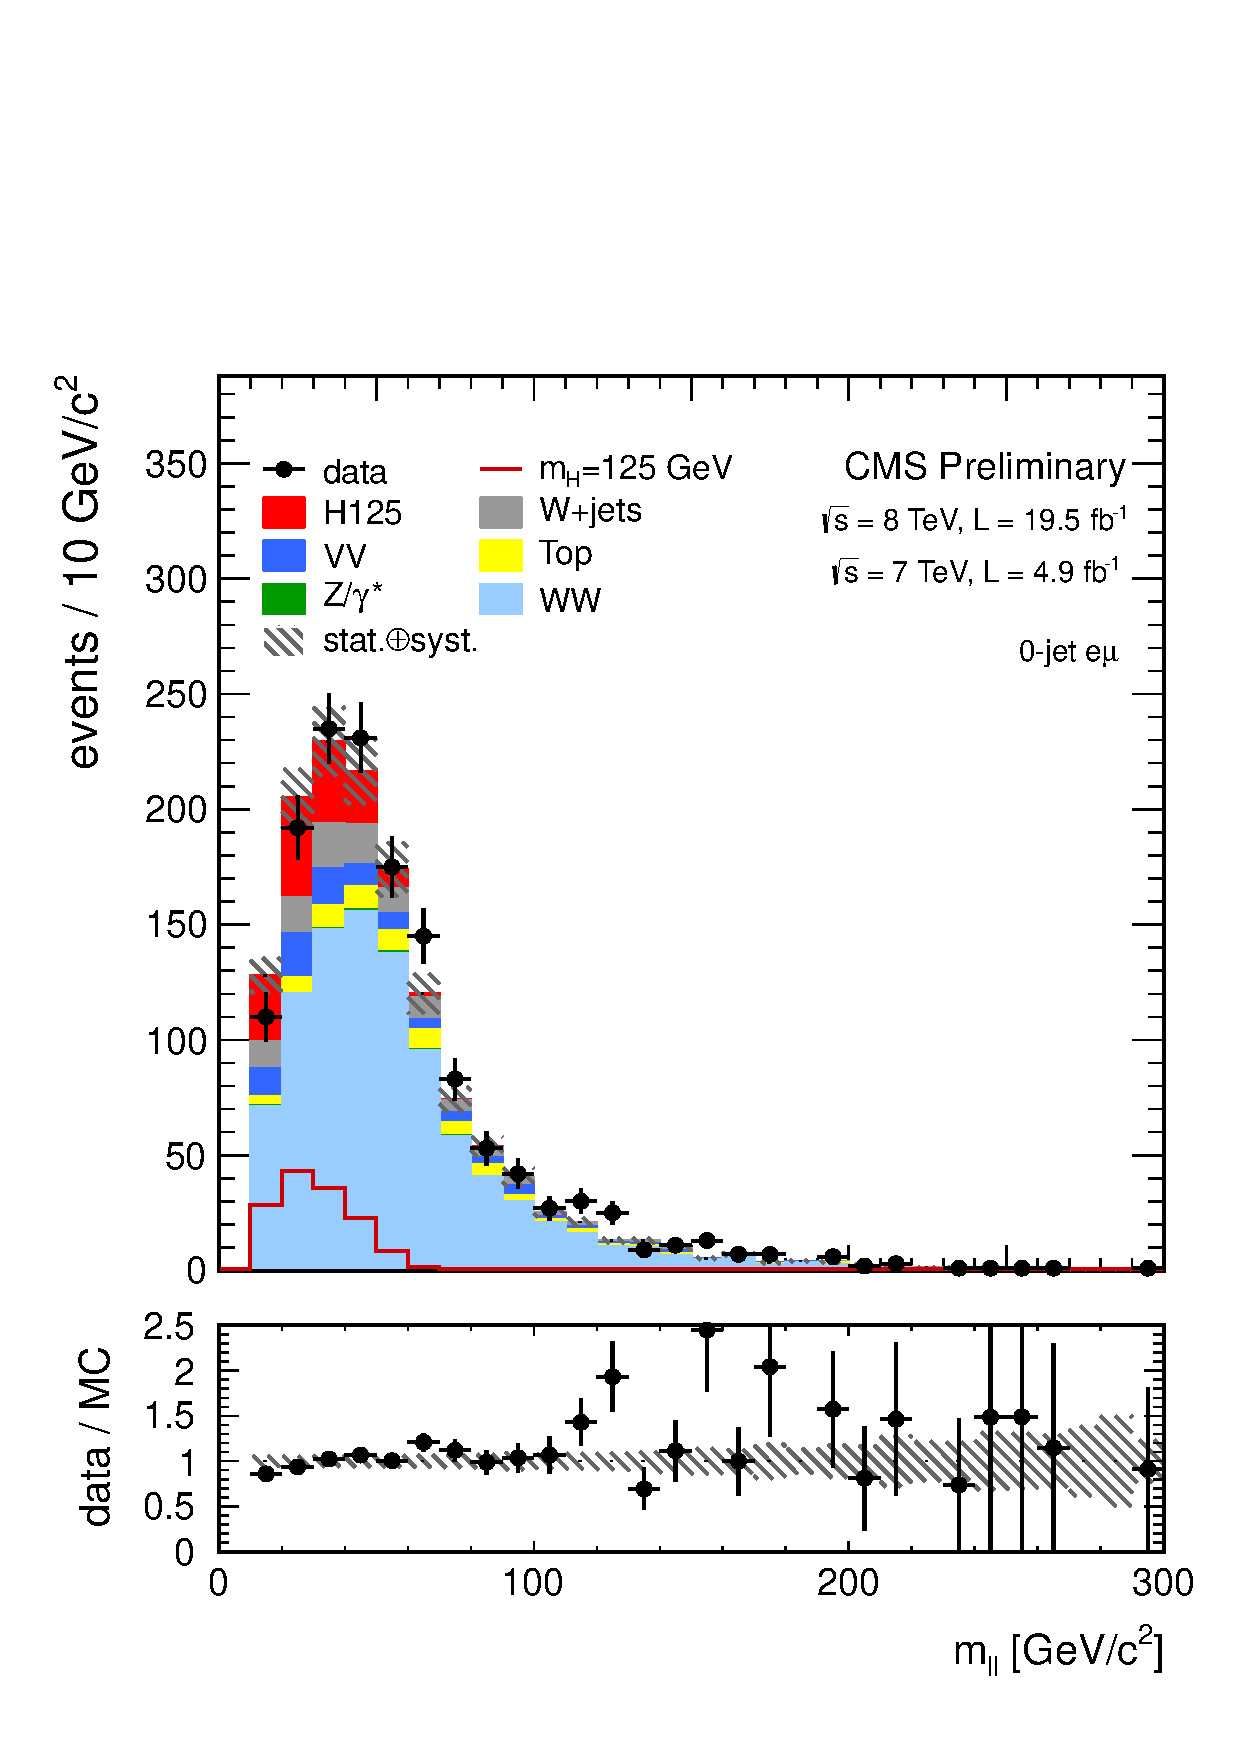
\includegraphics[width=0.49\textwidth,height=0.32\textheight]{mll_0j_of_nomll_Hsel_mll_Lin.pdf}
    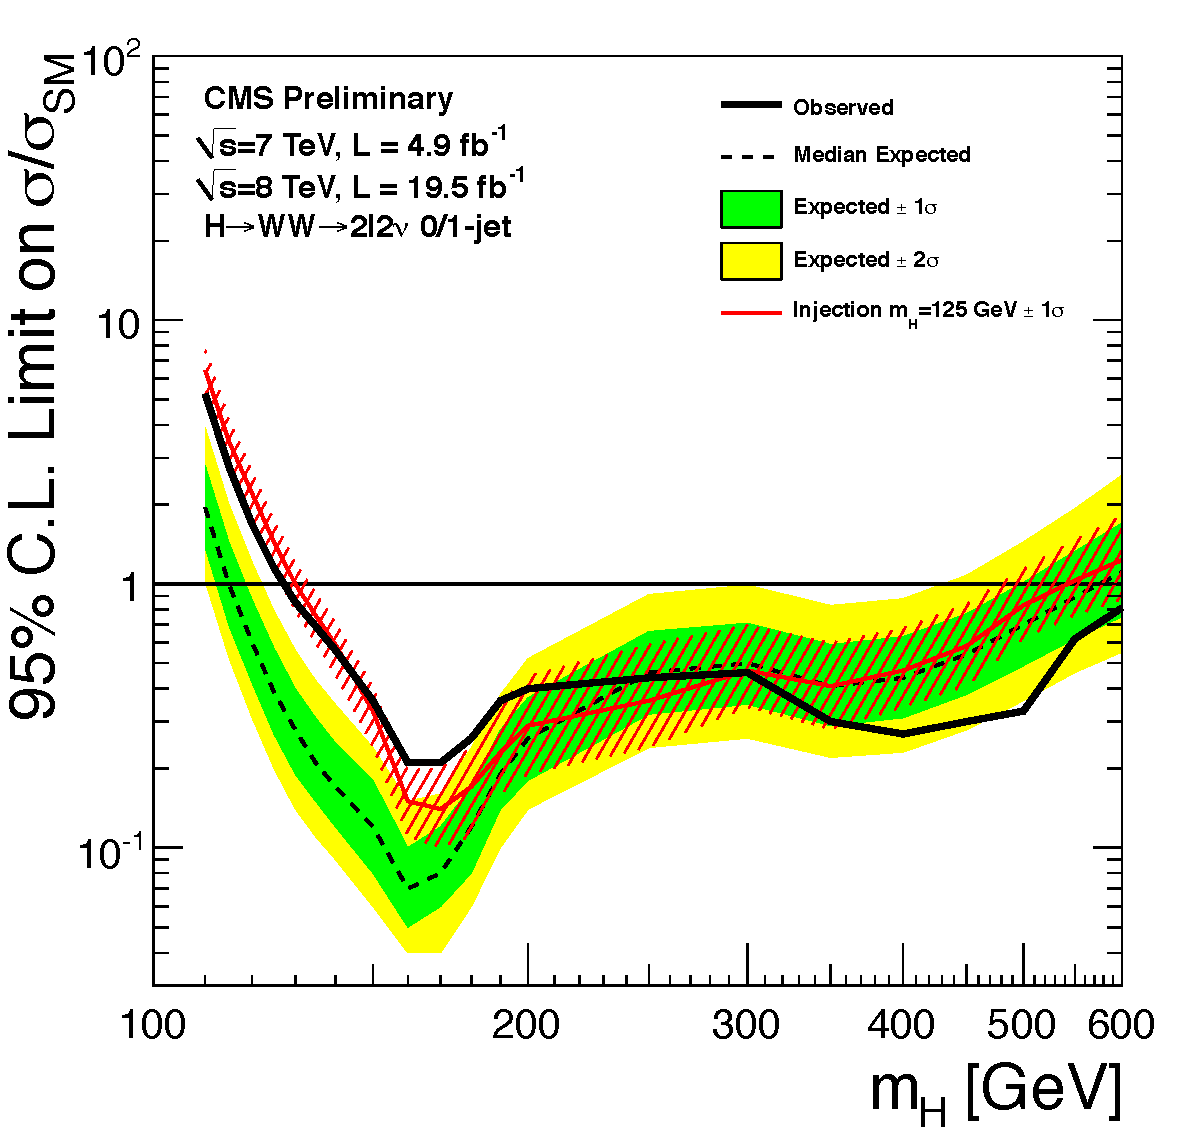
\includegraphics[width=0.49\textwidth,height=0.32\textheight]{limit_7p8TeV_shape_from110to600_logx1_logy1.pdf}
      \caption{Left: Distributions of dilepton mass in the 0-jet
	different-flavor final state for a $\mH=125$ GeV SM Higgs
	boson and for the main backgrounds.  Right: Expected and
	observed 95\% CL upper limits on the cross section times
	branching fraction, relative to the SM Higgs expectation,
	using the 7+8 TeV data. The expected limits in the presence
	of the Higgs with $\mH = 125$ GeV and its associated
	uncertainty are also shown. \label{fig:hww1}} \end{center}
\end{figure}


%%%%%%%%%%%%%%%%%%%%%%%%%%%%%%%%%%%%%%%%%%%%%%%%%%%%%%%%%%%%%%%%%%%%%%%%%%%%%%%
\section{The $\hzzfl$ Channel}
\label{sec:hzzfl}
%%%%%%%%%%%%%%%%%%%%%%%%%%%%%%%%%%%%%%%%%%%%%%%%%%%%%%%%%%%%%%%%%%%%%%%%%%%%%%%

The $H \to ZZ \to 4\ell$ channel is the cleanest channel and it is
often referred as the ``golden channel''.  The signal consists of four
isolated leptons. For high mass both pairs of opposite charge and same
flavour leptons are consistent with Z decays while for lower masses at
least one of the pairs has lower mass.  The Higgs branching ratio for
this channel is rather small, approximately one per mille at high mass
and lower for masses below $2\times\MW$ but the background is very
small.  The mass resolution is very good and ranges between 1 and 2\%.
The \pt of the lower \pt leptons is rather small and one of the most
important features of the analysis is the achievement of a very high
lepton efficiency down to very low \pt.  The analysis is carried out
in the mass range [110--1000] GeV.

The backgrounds consist of an irreducible component, from continuum ZZ
production, which is estimated from simulation, and a reducible
background, referred as $\cPZ+X$, from $\cPZ\bbbar$, $\ttbar$,
$\cPZ+\text{light jets}$, $\PW\cPZ+\text{jets}$ processes, where at
least one of the leptons is misidentified, which is estimated from
data control samples. After the selection a good agreement is observed
with the SM backgound in the $m_{4\ell}>$160 GeV range, with the
exception of an excess of events, concentrated around 125 GeV
(Fig.~\ref{fig:hzz1}). To enhance the sensitivity to the signal, and
also to study the properties of the observed resonance, a matrix
element likelihood approach is used to construct a kinematic
discriminant ($K_D$) based on the probability ratio of the signal and
background hypotheses, $K_D = {\cal P_\mathrm{sig}}/({\cal
P_\mathrm{sig}}+{\cal P_\mathrm{bkg}})$, where the leading-order
matrix elements define the probabilities for each value of
$m_{4\ell}$~\cite{Chatrchyan:2012ufa}.  This information is added to
the $m_{4\ell}$ in the likelihood used to extract the signal.  To
achieve sensitivity to different production modes (gluon fusion or
VBF) the events are categorized according to the presence of two
jets. In this case a Fisher discriminant is calculated using the jets
kinematics, while the Higgs boson candidate $\PT/m_{4\ell}$ is used
for the rest of the events.  Figure~\ref{fig:hzz1} (right) shows the
local p-values, as a function of $\MH$, for the low mass range: the
minimum is reached around 125.8 GeV, and corresponds to a local
significance of $6.7\sigma$ (for an expectation of $7.2\sigma$). The
signal strength $\mu$, relative to the expectation for the SM Higgs
boson, is $\mu = 0.91^{+ 0.30}_{-0.24}$ at 125.8 GeV.

%%%%%%%%%%%%%%%%%%%%%%%
\begin{figure}[th!]
\begin{center}
\centerline{
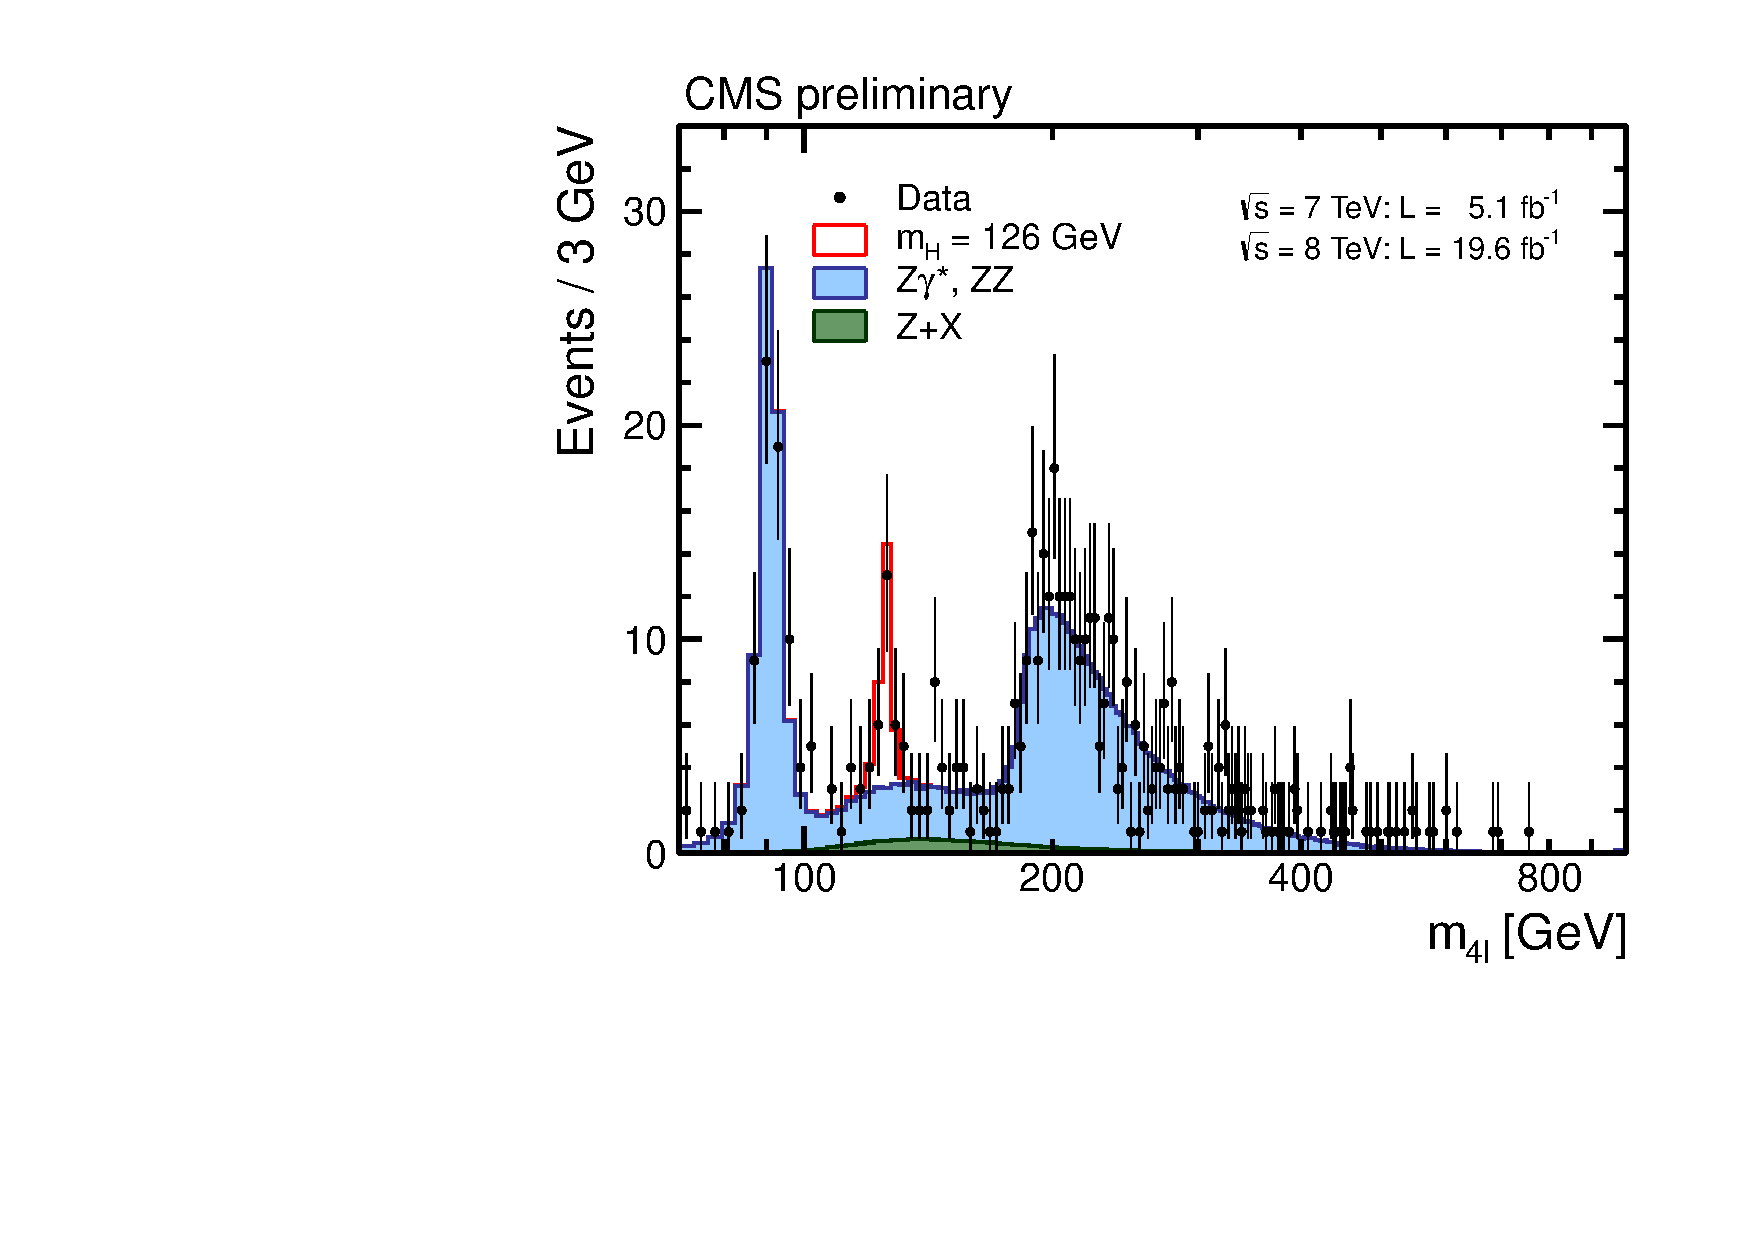
\includegraphics[width=0.5\linewidth,height=0.50\textwidth]{ZZMass_7Plus8TeV_70-1000_3GeV}
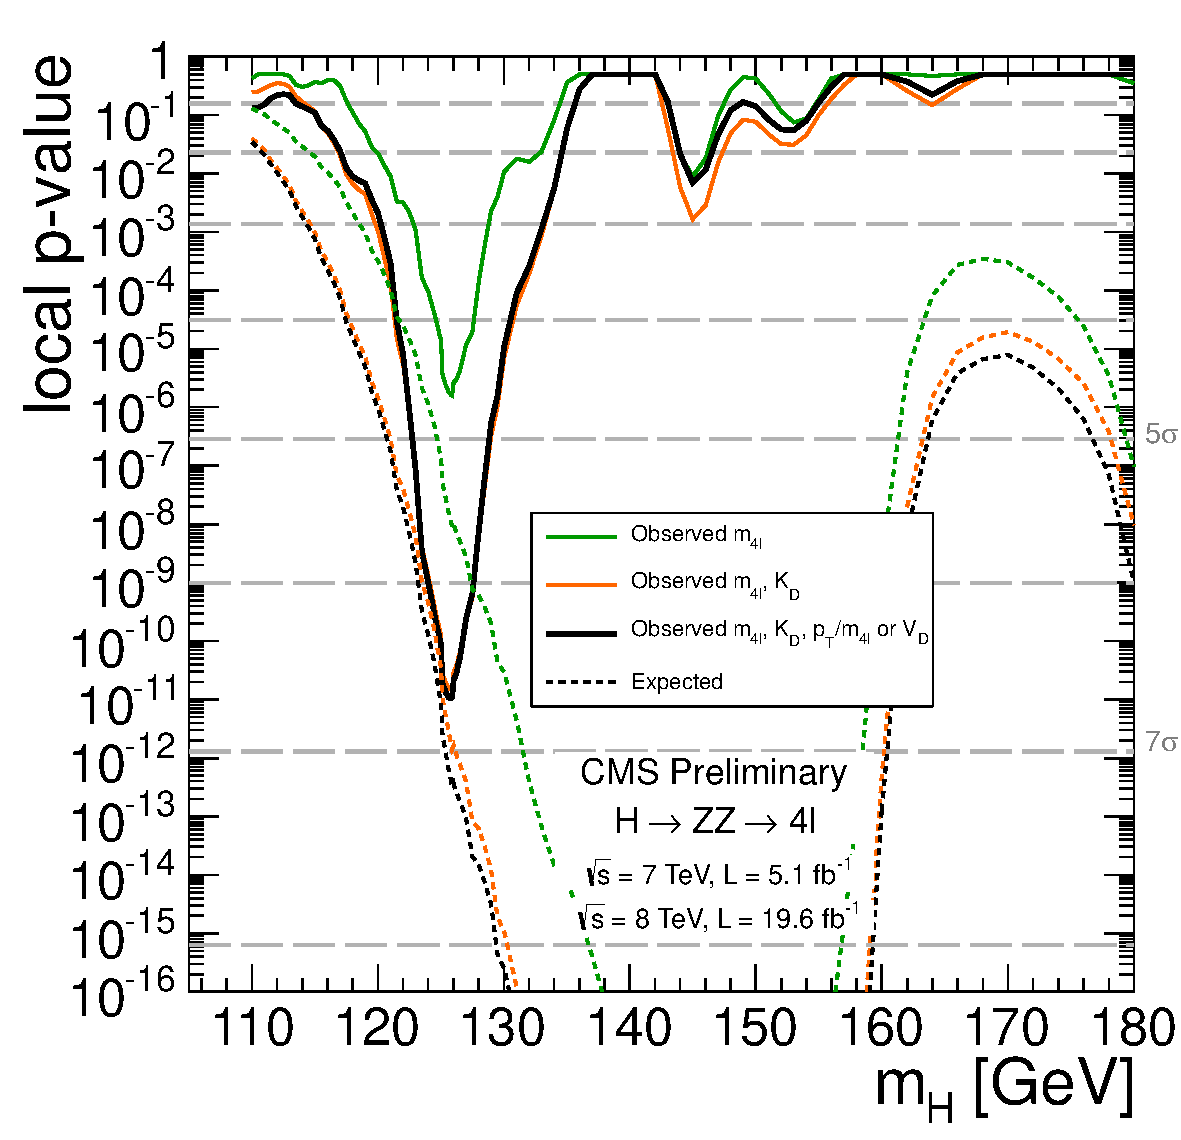
\includegraphics[width=0.5\linewidth,height=0.50\textwidth]{Pvals_PLP_lowMass_1D2D3D_Final3_no2l2tau_7p8sep}
}
\caption{Left: Distribution of the four-lepton reconstructed mass in the full mass range for the sum of 
the three $4\ell$ channels. Points represent the data, shaded
histograms represent the background and the unshaded histogram the
signal expectation.  Right: significance of the local excess with
respect to the SM background expectation as a function of the Higgs
boson mass (for $\MH<$180 GeV) for the 1D ($m_{4\ell}$), 2D
($m_{4\ell}$, $K_D$) and 3D ($m_{4\ell}$, $K_D$, $p_{T} /m_{4\ell}$ or
$V_D$) models.  }
\label{fig:hzz1}
\end{center}
\end{figure}
%%%%%%%%%%%%%%%%%%%%%%%

The mass measurement of the new resonance is performed with a
three-dimensional fit using for each event the $m_{4\ell}$, the
associated per-event mass error, and the $K_D$.  The resulting fit
gives $\mH$ = 125.8 $\pm$ 0.5 (stat.) $\pm$ 0.2 (syst.)~GeV.  The
systematic uncertainty accounts for the effect on the mass scale of
the lepton momentum scale and resolution.

To disentangle the production mechanisms of the new state (fermion
induced or vector boson induced), two signal strength modifiers
($\mu_F, \mu_V$) are introduced as scale factors to the SM expected
cross section. A two dimensional fit is performed for the two signal
strength modifiers assuming a mass hypothesis of $m_H = 125.8 \GeV$.
The ($\mu_V,\mu_F$) fit leads to the measurements $\mu_V =
1.0^{+2.4}_{-2.3}$ and $\mu_F = 0.9^{+0.5}_{-0.4}$ The measured values
are consistent with the expectations from the production of a SM Higgs
boson.

The spin and parity of the new state is also tested by constructing
discriminants using the probability ratio for two signal hypotheses
(SM and alternative). Six alternative models: $J^P=0^+, 0_h^+, 0^-,
2_{~mgg}^+, 2_{~mq\bar{q}}^+, 1^-, 1^+$ are considered. The
distribution of $q=-2{\ln({\cal L}_{J^P}/{\cal L}_{\rm SM})}$ is
examined with generated samples of background and signal of seven
types (SM $0^+$ and six $J^P$) for $m_H =126$ GeV. The data disfavours
the alternative hypotheses $J^P$ with a $\mathrm{CL_s}$ value in the
range 0.1--10\%. The measurement of the fraction of a $C\!P$-violating
contribution to the decay amplitude expressed through the fraction of
the corresponding decay rate is $f_{a3}=0.00^{+0.23}_{-0.00}$ or
equivalently $f_{a3}<0.58$ at 95\% CL.

\section{Conclusions}
\label{sec:Conclusions}

I have presented the results of the searches for the SM Higgs boson in
the $\hwwtl$ and $\hzzfl$ channels. The two channels both observe a
new state, with a cross section compatible with the SM Higgs boson.
The mass is measured with high precision in the four-lepton final
state: $\mH$ = 125.8 $\pm$ 0.5 (stat.) $\pm$ 0.2 (syst.)~GeV.  The
spin and parity of the new state are compatible with a SM Higgs boson.

\begin{thebibliography}{0}




\bibitem{Higgs1}{F. Englert and R. Brout}, \textit{ Phys. Rev. Lett.} \textbf{ 13} (1964) 321.
\bibitem{Higgs2}{P. W. Higgs}, \textit{ Phys. Rev. Lett.} \textbf{ 13} (1964) 508.
\bibitem{Chatrchyan:2012ufa} S.~Chatrchyan {\it et al.}, Phys.\ Lett.\ B {\bf 716}, 30 (2012)
\bibitem{Aad:2012tfa} G.~Aad {\it et al.}, Phys.\ Lett.\ B {\bf 716}, 1 (2012)
\bibitem{HWW2011} S.~Chatrchyan {\it et al.},  Phys.\ Lett.\ B {\bf 710}, 91 (2012)
\bibitem{antikt} M.~Cacciari, G.~P.~Salam and G.~Soyez, JHEP {\bf 0804}, 063 (2008)

\end{thebibliography}

\end{document}
\endinput
%%
%% End of file `cimsmple.tex'.
